\begin{samplecase}
{\bf Gamma-ray intensities: ${}^{208}$Pb$(n,n\gamma )$ and ${}^{208}$Pb$(n,2n\gamma )$}\newline
This feature could simply have been included in the sample case on 
excitation functions for ${}^{208}$Pb, but in order not to overburden the
description of that sample case we include it here. With the input file

\VerbatimInput{\samples n-Pb208-nngamma/org/talys.inp}

all discrete gamma lines are printed and stored in separate files.
To avoid the production of too many data files, we have put {\bf maxZ 0} so 
that only the gamma-ray production files for Pb-chain are created. Also, we 
include a special OMP with
the file {\em pb.omp} and we set {\bf isomer 1.e-4} to allow for gamma decay
of some rather short-lived levels.
Experimental data exists for 
the ${}^{208}$Pb$(n,n'\gamma)$ cross section for level 1 to level 0 and
the ${}^{208}$Pb$(n,2n'\gamma)$ cross section for level 2 to level 0 and for 
level 1 to level 0. These
data have been plotted together with the results of the calculated files
{\em gam082208L01L00.tot}, {\em gam082207L02L00.tot} and 
{\em gam082207L01L00.tot}, in Fig.~\ref{pbgamma}.

Here are the contents of {\em gam082207L01L00.tot} as an example:
{\small \begin{verbatim}

# header:
#   title: Pb208(n,xg_1-0)Pb207 gamma-ray production cross section
#   source: TALYS-2.0
#   user: Arjan Koning
#   date: 2023-12-11
#   format: YANDF-0.1
# target:
#   Z: 82
#   A: 208
#   nuclide: Pb208
# reaction:
#   type: (n,xg_1-0)
#   Q-value [MeV]: -7.937571E+00
#   E-threshold [MeV]:  7.976068E+00
#   level:
#     number: 1
#     energy [MeV]:  5.696980E-01
#     spin:  2.500000E+00
#     parity: -1
#     level:
#       number: 0
#       energy [MeV]:  0.000000E+00
#       spin:  5.000000E-01
#       parity: -1
#   gamma energy [MeV]:  5.696980E-01
# residual:
#   Z: 82
#   A: 207
#   nuclide: Pb207
# datablock:
#   quantity: gamma-ray production cross section
#   columns: 2
#   entries: 67
##       E             xs
##     [MeV]          [mb]
   1.000000E-11   0.000000E+00
.....................................
   7.500000E+00   0.000000E+00
   8.000000E+00   3.859060E-01
   8.500000E+00   9.522382E+01
   9.000000E+00   3.090241E+02
   9.500000E+00   5.028625E+02
   1.000000E+01   6.213652E+02
   1.100000E+01   7.397191E+02
   1.200000E+01   7.665779E+02
   1.300000E+01   7.781571E+02
   1.400000E+01   7.736282E+02
....................
\end{verbatim} } \renewcommand{\baselinestretch}{1.07}\small\normalsize
\noindent
\end{samplecase}
\begin{figure}
\centering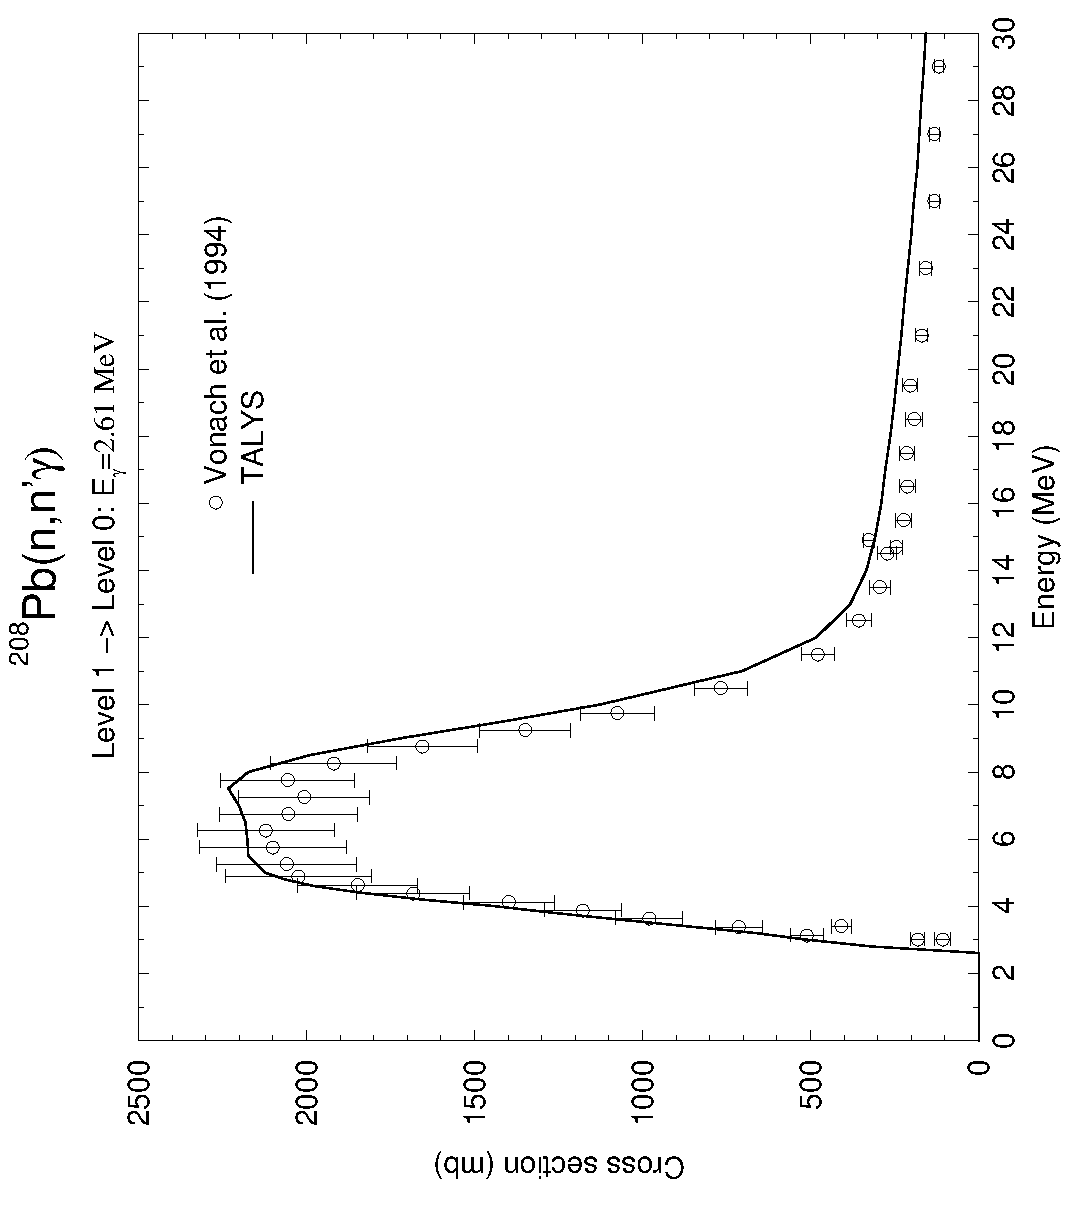
\includegraphics[scale=0.4,angle=270]{gam082208L01L00}
\centering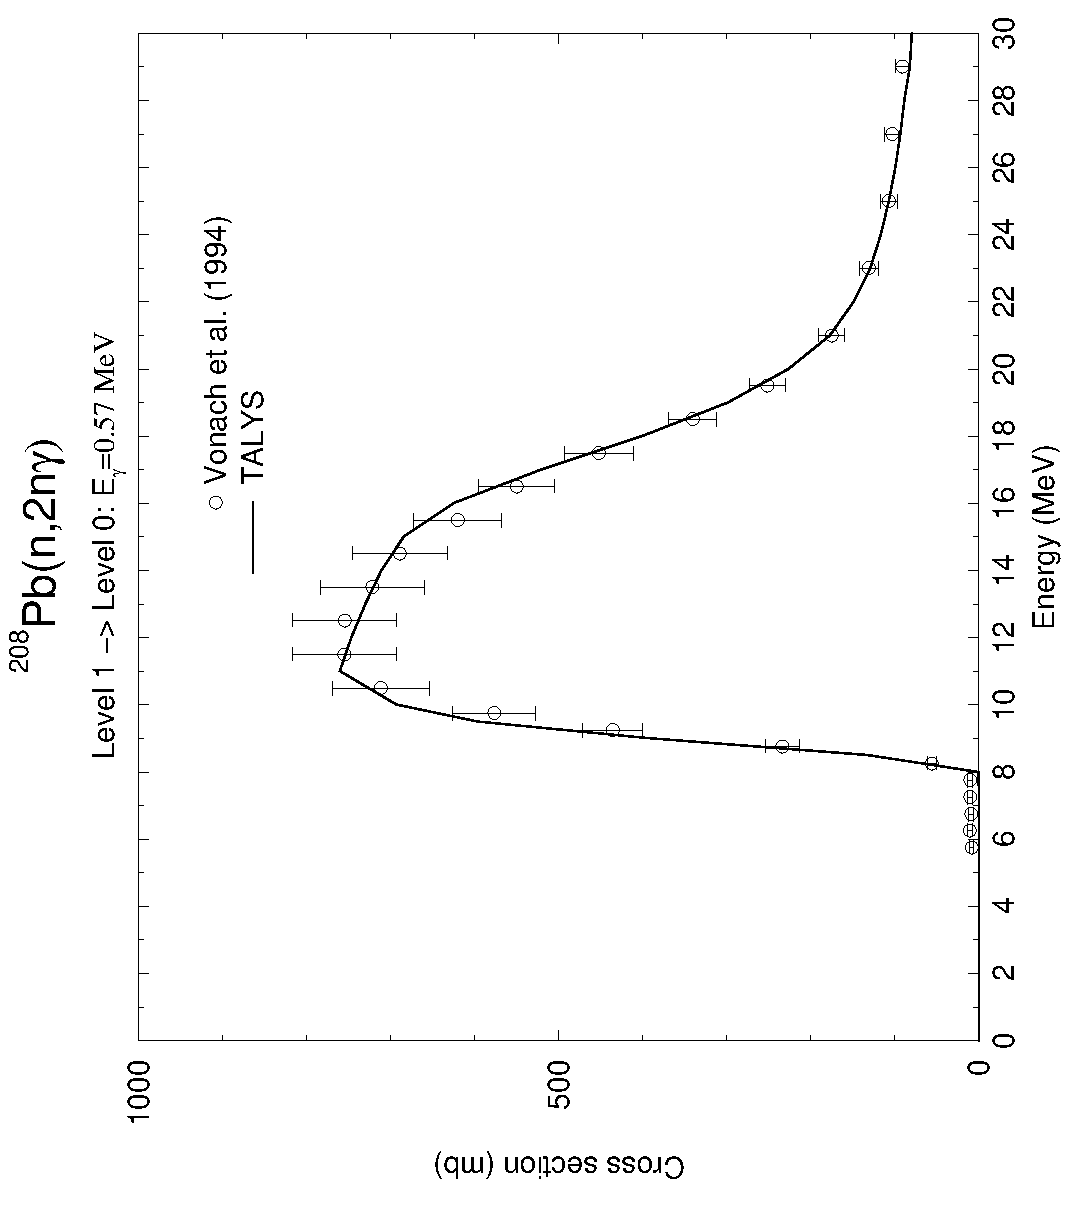
\includegraphics[scale=0.4,angle=270]{gam082207L01L00}
\centering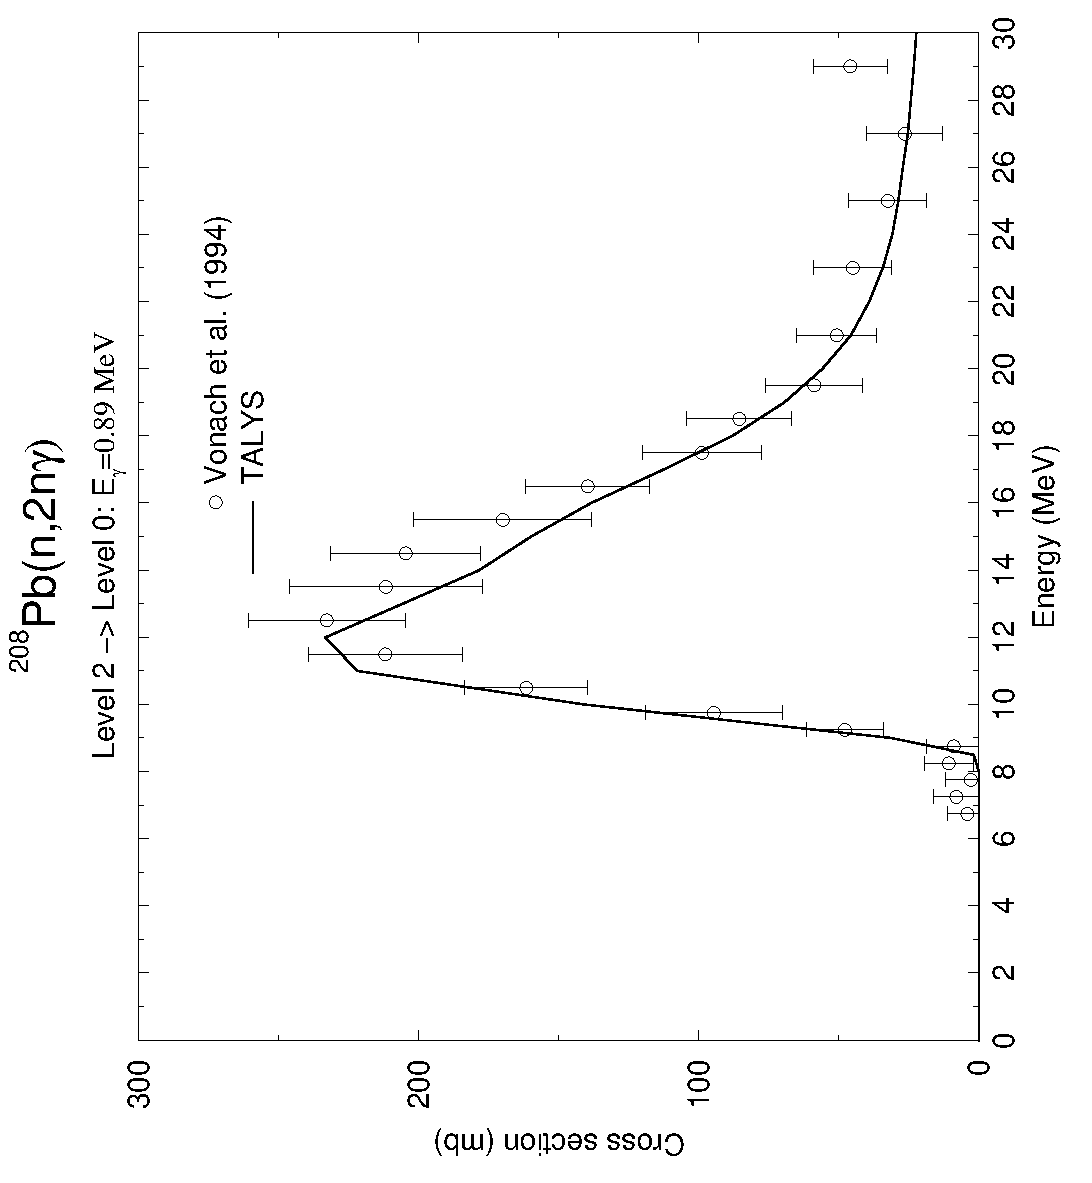
\includegraphics[scale=0.4,angle=270]{gam082207L02L00}
\caption{Gamma-ray production lines for a few transitions in ${}^{208}$Pb(n,n')
and ${}^{208}$Pb(n,2n) reactions.
The experimental data are from \protect\cite{Vonach1994}.}
\label{pbgamma}
\end{figure}

